% -*- coding: utf-8 -*-
\section{Density Functional Theory}

Having established the central importance of the electron density and its
relationship to physical observables, we now turn to a theoretical framework
where the electron density itself serves as the fundamental variable: Density
Functional Theory (DFT).

The idea of using the electronic density to extract information about a system
dates back to 1927, with the pioneering work of Llewellyn Hilleth Thomas and
Enrico Fermi~\cite{Thomas1927,fermi1927statistical}. Their approach involved
approximating the kinetic energy, along with the nucleus-electron and
electron-electron interactions, by modeling the system as a uniform electron
gas.

\follow{Thomas-Fermi Model}{

  Consider a hypothetical system with a constant electronic density:

  \begin{align}
    {T}_{\mathrm{TF}}[\rho(\mathbf{r})]=\displaystyle\frac{3}{10}(3\pi^2)^{\sfrac{2}{3}}\int
    \rho(\mathbf{r})^{\sfrac{5}{3}}\dd\tau
  \end{align}

  Combining this expression for the kinetic energy with classical electrostatic
  contributions leads to the total energy functional of the Thomas-Fermi model:

  \begin{align}
    {E}_{\mathrm{TF}}[\rho(\mathbf{r})]=\displaystyle\frac{3}{10}(3\pi^2)^{\sfrac{2}{3}}\int
    \rho(\mathbf{r})^{\sfrac{5}{3}}\dd\tau - Z\int\displaystyle\frac{\rho(\mathbf{r})}{r}\dd\tau
    +
    \displaystyle\frac{1}{2}\int\int\displaystyle\frac{\rho(\mathbf{r}_1)\rho(\mathbf{r}_2)}{r_{12}}
    \dd\tau_1\dd\tau_2
    \label{E_TF}
  \end{align}

}

This model describes the electronic structure using a density only weakly
confined by the nuclear potential. Although it neglects shell structure and
quantum interference effects, it performs reasonably well for alkali and
alkaline-earth metals, where valence electrons are loosely bound to the nuclei.

The Thomas-Fermi model is also noteworthy as a expression of the Copenhagen
interpretation of Quantum Mechanics.  This perspective laid the groundwork for
the formal development of \gls{DFT}, which advanced significantly with the
foundational theorems of Hohenberg and Kohn~\cite{Hohenberg1964}, and the
practical Kohn-Sham formalism introduced the following year~\cite{Kohn1965}.

\vfill%
\subsection{Hohenberg-Kohn Theorems~\cite{Hohenberg1964}}\label{HKteoremitas}
\subsubsection{Theorem 1}

The first Hohenberg-Kohn theorem asserts that the stationary ground-state electronic
density, $\rho(\mathbf{r})$, uniquely determines the external potential
$v_{\text{ext}}(\mathbf{r})$. Consequently, all
properties of the system ---including the Hamiltonian, the wavefunction, and the
total energy--- are uniquely determined by $\rho(\mathbf{r})$. Hence, two systems
of $N$ particles subject to distinct external potentials cannot exhibit the same
ground-state density, unless the potentials differ only by a constant.

\thm{HK's Theorem 1}{
  The ground-state expectation value of any observable $\widehat{A}$ is a unique
  functional of the exact ground-state density:
  \begin{align}
    \langle \psi |\widehat{A}|\psi \rangle = A[\rho_0 (\mathbf{r})]
  \end{align}
}

\cor{}{

  The external potential, and thus all ground-state properties of the system,
  are uniquely determined by the ground-state electronic density. This includes
  the many-body wavefunction. In particular, the \gls{HK} functional is
  defined as $F[\rho] = T[\rho] + U[\rho]$, a universal functional that is
  independent of the external potential.

}

\begin{figure}[H]
  % -*- coding: utf-8 -*-
%  ~VCastor 
\begin{tikzpicture}[>=Stealth, font=\sffamily]

  % === LABEL POSITIONS ===
  \coordinate (Vlabel) at (0,6);
  \coordinate (Psilabel) at (6,6);
  \coordinate (Rholabel) at (12,6);

  % === SPACE LABELS ===
  \node[font=\bfseries] at (Vlabel) {$V_{\mathrm{ext}}$};
  \node[font=\bfseries] at (Psilabel) {$\Psi$};
  \node[font=\bfseries] at (Rholabel) {$\rho$};

  % === Y OFFSET FOR BLOBS AND CONTENT ===
  \def\yshift{-0.5}

  % === IRREGULAR BLOBS ===
  \begin{scope}[shift={(Vlabel)}, yshift=\yshift cm, yscale=0.8]
    \draw[thick, draw=strongBlue, fill=pastelBlue, fill opacity=0.3]
      plot[smooth, tension=0.7]
      coordinates {(-2,-3.5) (-1.2,-1) (0.5,-0.2) (1.5,-1.2) (2,-2.5) (1.2,-3.5) (-1,-3.8) (-2,-3.5)};
  \end{scope}

  \begin{scope}[shift={(Psilabel)}, yshift=\yshift cm, yscale=0.8]
    \draw[thick, draw=strongPurple, fill=pastelPurple, fill opacity=0.3]
      plot[smooth, tension=0.7]
      coordinates {(-2,-3.5) (-1.5,-1.2) (0.2,-0.2) (1.2,-1.4) (2,-3.2) (1,-4.2) (-1,-4.5) (-2,-3.5)};
  \end{scope}

  \begin{scope}[shift={(Rholabel)}, yshift=\yshift cm, yscale=0.8]
    \draw[thick, draw=strongGreen, fill=pastelGreen, fill opacity=0.3]
      plot[smooth, tension=0.7]
      coordinates {(-2,-3.8) (-1,-1.5) (0.5,-0.5) (1.5,-1.7) (2,-3.5) (0.8,-4.3) (-1.2,-4.4) (-2,-3.8)};
  \end{scope}

  % === POINTS at mid-heights (~ -2.5) for aligned arrows ===
  \coordinate (V1) at ($(Vlabel)+(0,\yshift -1)$);
  \coordinate (V2) at ($(Vlabel)+(0,\yshift -2.2)$);
  \fill (V1) circle (2pt) node[left=2pt] {$v_\mathrm{ext}$};
  \fill (V2) circle (2pt) node[left=2pt] {$v_\mathrm{ext}^\prime$};

  \coordinate (Psi) at ($(Psilabel)+(0.5,\yshift -1.6)$);
  \fill (Psi) circle (2pt);

  \coordinate (Rho) at ($(Rholabel)+(0.3,\yshift -1.6)$);
  \fill (Rho) circle (2pt) node[right=2pt] {};

  % === VALID ARROWS: V -> rho ===
  \draw[->, thick] (V1) .. controls +(2,0.2) .. (Rho);
  \draw[->, thick] (V2) .. controls +(2,-0.2) .. (Rho);

  % === RED ARROWS: V -> Psi ===
  \draw[->, thick, red] (V1) -- (Psi);
  \draw[->, thick, red] (V2) -- (Psi);

  % === CTE ARROW ===
  \draw[<->, thick, draw=labelOrange] (V1) -- (V2)
    node[midway, left=4pt, text=labelOrange] {\textbf{cte}};

\end{tikzpicture}

  \caption{Hohenberg-Kohn Theorem 1. The red arrows point to the corresponding
    wavefunction, while the black arrows point directly to the density $\rho$.}
\end{figure}

\newpage
\subsubsection{Theorem 2}

The second Hohenberg-Kohn theorem establishes a variational principle for the
electron density. It states, for a given external potential
$v_{ext}(\mathbf{r})$ and electron number $N$, the ground-state energy
functional,
%
\begin{align}
  E_{v, N} [\rho] = F[\rho] + \int v_{ext}(\mathbf{r})\rho(\mathbf{r}) \dd\tau,
\end{align}

\noindent attains its minimum value when $\rho(\mathbf{r})$ is the exact ground-state
density. That is, among all physically admissible densities, the true
ground-state density yields the lowest energy.

\thm{HK's Theorem 2}{
  The ground-state energy is the minimum of the energy functional, providing a
  variational principle:
  %
  \begin{align}
    E_{0}\leq E[\rho]=T[\rho] + V_{Ne}[\rho]+V_{ee}[\rho]
  \end{align}
  with equality only when $\rho$ is the exact ground-state density.
}

\subsection{Kohn-Sham Approximation~\cite{Kohn1965}}\label{KSapprox}

Building on the Hohenberg-Kohn theorems, Kohn-Sham proposed a practical
scheme to address the many-electron problem by introducing an auxiliary system
of non-interacting particles that reproduces the exact ground-state electron
density of the fully interacting system. Within this framework, the total
energy of a system subject to an external potential $v_{\text{ext}}(\mathbf{r})$
is expressed as:
%
\begin{align}
  E[\rho(\mathbf{r})] = T_s[\rho(\mathbf{r})]
    + \int v_{ext}(\mathbf{r})\rho(\mathbf{r})\dd\tau
    + \frac12\int\int \frac{\rho(\mathbf{r})\rho(\mathbf{r}^{\,\prime})}{|\mathbf{r}-\mathbf{r}^{\,\prime}|}\dd\tau
    + E_{xc}[\rho(\mathbf{r})].
  \label{KS1}
\end{align}

In Equation~\ref{KS1}, the first term $T_s[\rho(\mathbf{r})]$ represents the
kinetic energy of the non-interacting reference electrons, the second term
corresponds to the interaction of the electrons with the external potential
(typically from the nuclei), the third is the classical Coulomb repulsion
(Hartree energy), and the last term captures all remaining quantum many-body
effects, which are encapsulated in the exchange-correlation functional
$E_{xc}[\rho(\mathbf{r})]$.

\newpage
To render the original interacting problem tractable, Kohn and Sham replaced
it with an equivalent, auxiliary non-interacting system moving in an effective
potential $v_\text{eff}(\mathbf{r})$, chosen such that it reproduces exactly
the ground-state density of the interacting electrons. The resulting
single-particle Kohn-Sham equation is:
%
\begin{align}
  \left (-\sfrac{1}{2}\nabla^2 + v_{eff}(\mathbf{r}) \right )
  \varphi_i = \epsilon_i \varphi_i,
\end{align}

\noindent where the effective potential $v_{\text{eff}}(\mathbf{r})$ acting on
the Kohn-Sham electrons is defined as: $v_{\text{eff}}(\mathbf{r}) =
v_{\text{ext}}(\mathbf{r}) + v_{\text{H}}(\mathbf{r}) + v_{xc}(\mathbf{r})$;
$v_\text{H}(\mathbf{r})$ is the classical Hartree potential arising from the
electron density:
$$v_\text{H}(\mathbf{r}) = \int
\frac{\rho(\mathbf{r}^{\,\prime})}
{|\mathbf{r}-\mathbf{r}^{\,\prime}|}\dd\tau^{\,\prime},$$
and $v_{xc}(\mathbf{r})$ is the exchange-correlation potential, defined as the
functional derivative of $E_{xc}[\rho(\mathbf{r})]$ with respect to the
density:
$$v_{xc}(\mathbf{r}) = \frac{\delta E_{xc}[\rho(\mathbf{r})]}{\delta\rho(\mathbf{r})}.$$

% \noindent where $v_{eff}$ denotes the effective potential acting on the
% non-interacting \gls{KS} electrons. It includes the external potential
% $v_\text{ext}$, the Hartree potential $v_\text{H}$, and the
% exchange-correlation potential $v_{\text{xc}}$. This potential ensures that the
% \gls{KS} system reproduces the ground-state density of the interacting system.

The exchange-correlation functional, $E_{xc}[\rho(\mathbf{r})]$, thus incorporates all
many-body effects beyond the classical electrostatic interaction, including
exchange effects due to the antisymmetry of the wavefunction and dynamic
electron correlation. Formaly, it can be expressed as the difference between the
true interacting energy and the components already accounted for in the
Kohn-Sham formalism:
%
\begin{align}
  E_{xc}[\rho(\mathbf{r})] = T[\rho(\mathbf{r})] - T_s[\rho(\mathbf{r})] +
    V_{ee}[\rho(\mathbf{r})] - J[\rho(\mathbf{r})] ,
\end{align}

\noindent
where $T[\rho(\mathbf{r})]$ is the kinetic energy of the interacting system,
$T_s[\rho(\mathbf{r})]$ is the kinetic energy of the non-interacting system,
$V_{ee}[\rho(\mathbf{r})]$ is the true electron-electron interaction energy,
and $J[\rho(\mathbf{r})]$ is the classical Coulomb repulsion energy.

\newpage
\subsection{Exchange-Correlation Functionals}

As the exact analytical form of the universal exchange-correlation functional remains
unknown, \gls{DFT} relies on approximate models to capture many-body exchange
and correlation effects. Over the years, numerous functionals have been
developed, varying in both complexity and accuracy.

To organise this diversity, functionals are often placed within the conceptual
framework of Jacob's ladder (Figure~\ref{ladder_eye}), which symbolically
depicts the climb toward chemical accuracy through successive levels of
approximation. Each rung introduces additional physical ingredients ---such as
density gradients or explicit orbital dependence--- with the goal of
systematically improving the treatment of electron
interactions~\cite{Perdew2001}. In what follows, we briefly review the main
levels of this hierarchy.

\begin{figure}[H]
  \centering
  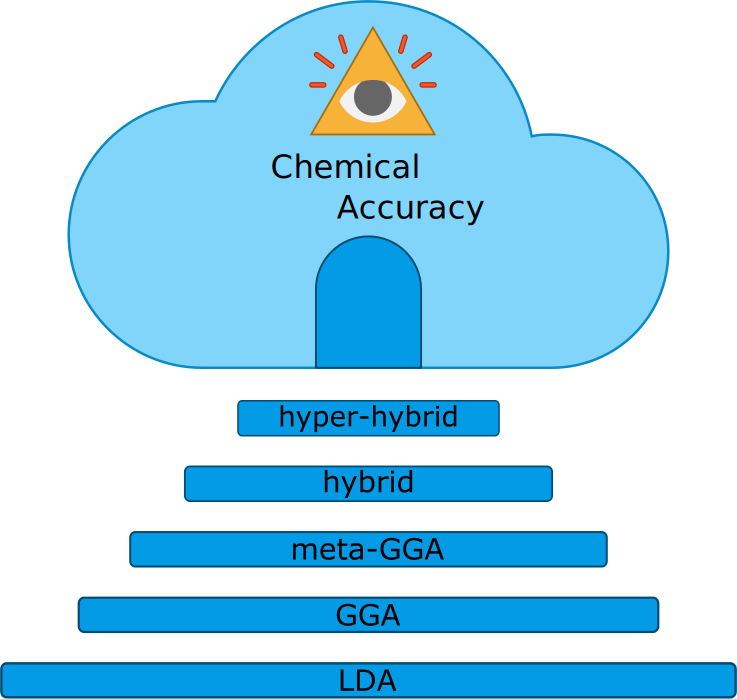
\includegraphics[width=0.45\textwidth]{img/heaven.pdf}
  \caption{The rungs of the
    ladder represent different levels of approximation, with each level
    incorporating additional physical effects to improve accuracy.}
  \label{ladder_eye}
\end{figure}

\nt{
  \paragraph{Double-Hybrid} It is important to note that, although double-hybrids
  are placed on the fifth rung of Jacob's ladder, they are not obtained by merely
  adding an extra density-dependent term to a functional. In practice, a
  double-hybrid combines a fraction of \gls{HF}-like exchange with a second-order
  perturbative correlation contribution evaluated with \gls{KS} orbitals (often
  ``MP2-like''). The latter requires access to virtual orbitals and orbital
  energy differences and is typically
  evaluated in a post-SCF step~\cite{Goerigk2014}.
  % with a $\mathcal{O}(N^5)$ scaling
}

\newpage
\begin{itemize}

  \item \textbf{Local Density Approximation (LDA).} In the \gls{LDA}, the
  electron density is locally approximated as a homogeneous electron gas with
  density $\rho$. In this model, the electrons are immersed in a uniform
  background of positive charge, forming an electrically neutral system with
  infinite volume and an infinite number of non-interacting
  electrons~\cite{Koch2001}.

  The corresponding exchange-correlation energy functional is written as:

  $E_{xc}^{LDA}[\rho] = \int\rho(\mathbf{r}) \varepsilon_{xc}(\rho(\mathbf{r}))\dd\tau$

  Taking the functional derivative with respect to the density yields the
  exchange-correlation potential:

  $v_{xc}^{LDA} = \fdv{E_{xc}^{LDA}}{\rho} = \varepsilon_{xc}(\rho(\mathbf{r}))
  + \rho \dv{\varepsilon_{xc}(\rho(\mathbf{r}))}{\rho}$

  The exchange-correlation energy per particle, $\varepsilon_{xc}$, can be split
  into exchange and correlation contributions. The exchange part is given by:

  $\varepsilon_{x} = -\frac34 \left(\frac3\pi\right)^{\sfrac{1}{3}}\rho^{\sfrac{1}{3}}$ 

  Several variants of the \gls{LDA} have been developed to improve accuracy. The
  X$_\alpha$ method~\cite{Slater74} introduces an empirical parameter $\alpha$ to
  scale the exchange term. The Local Spin Density Approximation
  (LSDA)~\cite{Slater74} extends the LDA to spin-polarised systems by treating
  the spin-up and spin-down densities, $\rho_\alpha$ and $\rho_\beta$, separately.

  While an analytical form for the correlation energy $\varepsilon_{cor}$ is not
  available, several parameterisations based on Quantum Monte Carlo data have
  been proposed. The VWN functional~\cite{Vosko1980} was derived from simulations
  by Vosko, Wilk, and Nusair. Another important development was made by Perdew and
  Zunger, who fitted an analytic expression to Quantum Monte Carlo data obtained
  by Ceperley and Alder~\cite{Ceperley1980}, producing the widely used PL
  functional~\cite{Perdew1981}, which satisfies exact limits at both low and high
  densities.

  % \pagebreak
  \newpage
  %
  \item \textbf{Generalised Gradient Approximation (GGA).} The \gls{GGA} improves
  upon the constant-density assumption of the LDA by incorporating the gradient
  of the electron density into the functional form. This allows GGA functionals to
  account for the inhomogeneity of the electron distribution more accurately.

  The general form of a GGA exchange-correlation functional is:

  $E_{xc}^{GGA} [\rho] = \int\rho(\mathbf{r}) \varepsilon_{xc}(\rho(\mathbf{r}), \nnabla\rho(\mathbf{r})) \dd\tau$

  As in the \gls{LDA}, the exchange-correlation energy in the \gls{GGA} framework is typically
  decomposed into separate exchange and correlation contributions. Various strategies
  have been developed to incorporate the density gradient. One influential approach,
  introduced by Becke, is based on the concept of the exchange hole. Among the
  functionals derived from this idea, the B88 exchange functional~\cite{Becke1988}
  is one of the most widely used.

  Some \gls{GGA} functionals have been constructed as refinements of earlier GGAs. For
  example, the modified Perdew--Wang functional (mPW)~\cite{Adamo1998} improves the
  long-range behaviour of the exchange term relative to its predecessors.


  The B88 exchange functional is often paired with the LYP correlation functional,
  developed by Lee, Yang, and Parr~\cite{Lee1988}. LYP is based on a transformation
  of the Colle-Salvetti correlation energy~\cite{Colle1975}, originally derived for
  closed-shell systems, and incorporates the Weizsäcker kinetic energy
  term~\cite{weizsacker1935theorie} to improve accuracy in regions of rapid density
  variation.

  Another notable \gls{GGA} functional is P86~\cite{Perdew1986}, which is built
  upon the idea of a natural separation between exchange and correlation. It
  recovers the gradient expansion for slowly varying densities and incorporates
  uniform-gas and inhomogeneity effects beyond the random phase approximation.
  Importantly, the gradient-dependent terms vanish for uniform densities,
  ensuring that the functional reduces to the local form in the homogeneous
  limit.

  %
  \newpage
  \item \textbf{Meta-Generalised Gradient Approximation (meta-GGA).} The
  meta-GGA class of functionals extends the \gls{GGA} by including higher-order
  derivatives of the density, such as the Laplacian $\nabla^2\rho(\mathbf{r})$
  ---in practice the kinetic energy density $\tau(\mathbf{r})$--- which provides
  a measure of the localisation of the \gls{KS} orbitals.

  The kinetic energy density is defined as:

  $\tau^L(\mathbf{r}) = -\sfrac{1}{2} \displaystyle\sum_i^N \varphi_i^*(\mathbf{r})\nabla^2\varphi_i(\mathbf{r})$

  This leads to the general form of a meta-GGA exchange--correlation
  functional:

  $E_{xc}^{mGGA} [\rho] =
    \int\rho(\mathbf{r}) \varepsilon_{xc}(\rho(\mathbf{r}), \nnabla\rho(\mathbf{r}), \tau(\mathbf{r})) \dd\tau$

  The kinetic energy density and the Laplacian are connected through the
  external potential via the relation:

  %% Corect the eqution
  $\tau(\mathbf{r}) = \sfrac{1}{2}\displaystyle\sum_i^N |\nnabla\varphi_i(\mathbf{r})|^2
    - \sfrac{1}{4} \nabla^2\rho(\mathbf{r})$

  Although computing the Laplacian is more demanding and early meta-GGA
  functionals offered only modest improvements over \gls{GGA}, recent developments
  ---notably the SCAN functional~\cite{scan}--- have shown significant gains in
  accuracy, especially for systems with varying degrees of localisation and
  inhomogeneity.

  Two well-known examples of meta-GGA functionals are: $i$) the VSXC
  functional~\cite{VanVoorhis1998}, which is based on the density matrix
  expansion, and $ii$) the KCIS functional~\cite{kcis1999}, which introduces a
  self-interaction-corrected correlation energy and a gap in the uniform electron
  gas.

  %
  \newpage
  \item \textbf{Hybrid Functionals.} Hybrid functionals incorporate a fraction of
  exact exchange energy (\gls{HF}-like level), using the
  \gls{KS} orbitals. This combination enhances the accuracy of exchange
  interactions, particularly in systems where self-interaction errors are
  significant.

  The Hartree-Fock exchange energy is given by:

  $E_x^{HF} = -\sfrac{1}{2}\displaystyle\sum_{i,j}^N\displaystyle\int
  \displaystyle\frac{\varphi_{i}^{\star}(\mathbf{r}_1)
    \varphi_j^{\star}(\mathbf{r}_1) \varphi_i(\mathbf{r}_2) \varphi_j(\mathbf{r}_2)}
    {r_{12}} \dd\tau_1 \dd\tau_2$

  One of the most widely used hybrid functionals is B3LYP, developed in 1994 by
  combining Becke's three-parameter exchange functional~\cite{Becke1993} with the
  LYP correlation functional~\cite{Lee1988}. Its form is given by:

  $E_{xc}^{B3LYP} = aE_{x}^{Slater} + (1-a)E_x^{HF} +bE_x^{Becke88}
  +cE_c^{LYP} + (1-c)E_c^{VWN}$,

  where the parameters ($a = 0.80$, $b = 0.72$, and $c = 0.81$) were empirically
  determined to reproduce experimental values such as ionisation energies,
  atomisation enthalpies, proton affinities, and atomic energies.

  Other notable hybrid functionals include PBE0~\cite{Adamo1999}, which blends
  25 \% exact \gls{HF} exchange with 75 \% \gls{DFT} exchange from the
  PBE functional~\cite{Ernzerhof1998}, resulting in a well-balanced formulation.
  Another widely used example is M06-2X~\cite{Zhao2007}, a meta-GGA hybrid
  designed to improve accuracy in modelling non-covalent interactions,
  thermochemistry, and reaction barrier heights.

\end{itemize}

% -------------------------
\subimport{./}{functionals}

\newpage
\subsection{Computational implementation}

All the theoretical considerations discussed so far are not only mathematically
intriguing, but also offer deep insights into the physical nature of electronic
systems. However, it is equally important to understand how these ideas are
implemented computationally and whether their solutions are practically
tractable.

Fortunately, the \gls{SCF} algorithm, originally developed for \gls{HF} theory,
can be readily adapted for \gls{DFT} calculations~\cite{Kohn1965,Engel2011}. By
incorporating exchange-correlation effects into the Fock matrix, the \gls{SCF}
procedure becomes compatible with any chosen exchange-correlation functional.

The Fock matrix, which in the \gls{HF} formalism depends on the core
Hamiltonian, the Coulomb, and exchange
integrals, expressed as:
%
\begin{align}
  \mFock = \mFock(\Ha^{\mathrm{core}},\, J,\, K),
\end{align}

\noindent can be modified at the \gls{DFT} level by replacing the
\gls{HF} exchange term with the exchange-correlation contribution:
%
\begin{align}
  \mFock = \mFock(\Ha^{\mathrm{core}},\, J,\, \mFock^{\mathrm{XC}}).
\end{align}

\noindent The exchange-correlation component of the Fock matrix for a given
functional $f$ takes the general form:
%
\keq{}{
  \begin{align}
    \mFock_{\mu\nu}^{\mathrm{XC}\alpha} =
    \int\left[ \pdv{f}{\rho_\alpha}\phi_\mu\phi_\nu +
      \left( 2\pdv{f}{\gamma_{\alpha\alpha}}\nnabla\rho_\alpha
        + \pdv{f}{\gamma_{\alpha\beta}}\nnabla\rho_\beta \right)
    \cdot \nnabla\phi_\mu\phi_\nu \right] \dd\tau.
  \end{align}
}

This formulation allows exchange-correlation effects to be fully
embedded within the \gls{SCF} algorithm, as described earlier in
Section~\ref{HF_sec}.

\newpage

